% done

\chapter{\IFRU{Поиск в коде того что нужно}{Finding important/interesting stuff in the code}}

\IFRU{Современный софт, в общем-то, минимализмом не отличается.}{Minimalism it's not a significant feature
of modern software.}

\IFRU{Но не потому, что программисты слишком много написали, 
а потому что к исполняемым файлам обыкновенно прикомпиливают все подряд библиотеки. 
Если бы все вспомогательные библиотеки всегда выносили во внешние DLL, мир был бы иным.
(Еще одна причина для Си++ - STL и прочие библиотеки шаблонов.)}
{But not because programmers wrote a lot, but because all libraries are usually linked statically
to executable files.
If all external libraries were shifted into external DLL files, the world would be different.
(Another reason for C++ - STL and other template libraries.)}

\newcommand{\FOOTNOTEBOOST}{\footnote{\url{http://www.boost.org/}}}
\newcommand{\FOOTNOTELIBPNG}{\footnote{\url{http://www.libpng.org/pub/png/libpng.html}}}

\IFRU{Таким образом, очень полезно сразу понимать, какая функция из стандартной библиотеки или 
более-менее известной (как Boost\FOOTNOTEBOOST, libpng\FOOTNOTELIBPNG), 
а какая ~--- имеет отношение к тому что мы пытаемся найти в коде.}
{Thus, it's very important to determine origin of some function, if it's from standard library or 
well-known library (like Boost\FOOTNOTEBOOST, libpng\FOOTNOTELIBPNG),
and which one ~--- is related to what we are trying to find in the code.}

\IFRU{Переписывать весь код на \CCpp, чтобы разобраться в нем, безусловно, не имеет никакого смысла.}
{It's just absurdly to rewrite all code to \CCpp to find what we looking for.}

\IFRU{Одна из задач reverse engineer-а это быстрый поиск в коде того что собственно его интересует.}
{One of the primary reverse engineer's task is to find quickly in the code what is needed.}

\IFRU{Дизассемблер \IDA позволяет делать поиск как минимум строк, последовательностей байт, констант.
Можно даже сделать экспорт кода в текстовый файл .lst или .asm и затем натравить на него \TT{grep}, \TT{awk}, итд.}
{\IDA disassembler can search among text strings, byte sequences, constants.
It's even possible to export the code into .lst or .asm text file and then use \TT{grep}, \TT{awk}, etc.}

\IFRU{Когда вы пытаетесь понять, что делает тот или иной код, это запросто может быть какая-то 
опенсорсная библиотека вроде libpng. Поэтому когда находите константы, или текстовые строки которые 
выглядят явно знакомыми, всегда полезно их погуглить.
А если вы найдете искомый опенсорсный проект где это используется, 
то тогда будет достаточно будет просто сравнить вашу функцию с ней. 
Это решит часть проблем.}
{When you try to understand what some code is doing, this easily could be some open-source library like libpng.
So when you see some constants or text strings looks familiar, it's always worth to google it.
And if you find the opensource project where it's used, 
then it will be enough just to compare the functions. It may solve some part of problem.}

\IFRU{К примеру, однажды я пытался разобраться как происходит компрессия/декомпрессия сетевых пакетов в SAP 6.0. 
Это очень большая программа, но к ней идет подробный .PDB-файл с отладочной информацией, и это очень удобно. 
Я в конце концов пришел к тому что одна из функций декомпрессирующая пакеты называется CsDecomprLZC(). 
Не сильно раздумывая, я решил погуглить и оказалось что функция с таким же названием имеется в MaxDB
(это опен-сорсный проект SAP)\footnote{Больше об этом в соответствующей секции~\ref{sec:SAPGUI}}.}
{For example, once upon a time I tried to understand how SAP 6.0 network packets compression/decompression 
is working.
It's a huge software, but a detailed .PDB with debugging information is present, and that's cosily.
I finally came to idea that one of the functions doing decompressing of network packet called CsDecomprLZC().
Immediately I tried to google its name and I quickly found that the function named as the same is used in MaxDB
(it's open-source SAP project)\footnote{More about it in releval section~\ref{sec:SAPGUI}}.}

\url{http://www.google.com/search?q=CsDecomprLZC}

\IFRU{Каково же было мое удивление, когда оказалось, что в MaxDB используется точно такой же алгоритм, 
скорее всего, с таким же исходником.}
{Astoundingly, MaxDB and SAP 6.0 software shared the same code for network packets compression/decompression.}

\section{\IFRU{Связь с внешним миром}{Communication with the outer world}}

\IFRU{Первое на что нужно обратить внимание, это какие функции из API операционной 
системы и какие функции стандартных библиотек используются.}
{First what to look on is which functions from operation system API and standard libraries are used.}

\IFRU{Если программа поделена на главный исполняемый файл и группу DLL-файлов, 
то имена функций в этих DLL, бывает так, могут помочь.}
{If the program is divided into main executable file and a group of DLL-files, sometimes,
these function's names may be helpful.}

\IFRU{Если нас интересует, что именно приводит к вызову \TT{MessageBox()} с определенным текстом, 
то первое что можно попробовать сделать: найти в сегменте данных этот текст, найти ссылки на него, и найти, 
откуда может передаться управление к интересующему нас вызову \TT{MessageBox()}.}
{If we are interesting, what exactly may lead to \TT{MessageBox()} call with specific text,
first what we can try to do: find this text in data segment, find references to it and find the points
from which a control may be passed to \TT{MessageBox()} call we're interesting in.}

\IFRU{Если речь идет об игре, и нам интересно какие события в ней более-менее случайны, 
мы можем найти функцию \rand или её заменитель (как алгоритм Mersenne twister), и посмотреть, 
из каких мест эта функция вызывается и что самое главное: как используется результат этой функции.}
{If we are talking about some game and we're interesting, which events are more or less random in it,
we may try to find \rand function or its replacement (like Mersenne twister algorithm) and find a places
from which this function called and most important: how the results are used.}

\IFRU{Но если это не игра, а \rand используется, то также весьма любопытно, зачем. 
Бывают неожиданные случаи вроде использования \rand в алгоритме для сжатия данных (для имитации шифрования):}
{But if it's not a game, but \rand is used, it's also interesing, why.
There are cases of unexpected \rand usage in data compression algorithm (for encryption imitation):}
\url{http://blog.yurichev.com/node/44}.

\section{\IFRU{Строки}{String}}

\IFRU{Очень сильно помогают отладочные сообщения, если они имеются. В некотором смысле, отладочные сообщения, 
это отчет о том, что сейчас происходит в программе. Зачастую, это \printf-подобные функции, 
которые пишут куда-нибудь в лог, а бывает так что и не пишут ничего, но вызовы остались, так как эта сборка ~--- 
не отладочная, а release.}
{Debugging messages are often very helpful if present. In some sense, debugging messages are reporting
about what's going on in program right now. Often these are \printf-like functions,
which writes to log-files, and sometimes, not writing anything but calls are still present, because this build
is not debug build but release one.}
\IFRU{Если в отладочных сообщениях дампятся значения некоторых локальных или глобальных переменных, 
это тоже может помочь, как минимум, узнать их имена. 
Например, в Oracle RDBMS одна из таких функций: \TT{ksdwrt()}.}
{If local or global variables are dumped in debugging messages, it might be helpful as well because it's 
possible to get variable names at least.
For example, one of such functions in Oracle RDBMS is \TT{ksdwrt()}.}

\IFRU{Может также помочь наличие \TT{assert()} в коде: обычно этот макрос оставляет название файла-исходника, 
номер строки, и условие.}
{Sometimes \TT{assert()} macro presence is useful too: usually, this macro leave in code source file name, 
line number and condition.}

\newcommand{\CONUSONE}{http://blog.yurichev.com/node/32}
\newcommand{\CONUSTWO}{http://blog.yurichev.com/node/43}

\IFRU{Осмысленные текстовые строки вообще очень сильно могут помочь. 
Дизассемблер \IDA может сразу указать, из какой функции и из какого её места используется эта строка. 
Попадаются и \href{\CONUSONE}{смешные случаи}.}
{Meaningful text strings are often helpful.
\IDA disassembler may show from which function and from which point this specific string is used.
Funny cases \href{\CONUSONE}{sometimes happen}.}

\IFRU{Парадоксально, но сообщения об ошибках также могут помочь найти то что нужно. 
В Oracle RDBMS сигнализация об ошибках проходит при помощи вызова некоторой группы функций. 
\href{\CONUSTWO}{Тут еще немного об этом}.}
{Paradoxically, but error messages may help us as well.
In Oracle RDBMS, errors are reporting using group of functions.
\href{\CONUSTWO}{More about it}.}

\IFRU{Можно довольно быстро найти, какие функции сообщают о каких ошибках, и при каких условиях.}
{It's possible to find very quickly, which functions reporting about errors and in which conditions.}
\IFRU{Это, кстати, одна из причин, почему в защите софта от копирования, 
бывает так, что сообщение об ошибке заменяется 
невнятным кодом или номером ошибки. Мало кому приятно, если взломщик быстро поймет, 
из за чего именно срабатывает защита от копирования, просто по сообщению об ошибке.}
{By the way, it's often a reason why copy-protection systems has inarticulate cryptic error messages 
or just error numbers. No one happy when software cracker quickly understand why copy-protection
is triggered just by error message.}

\section{\IFRU{Константы}{Constants}}

\IFRU{Некоторые алгоритмы, особенно криптографические, используют хорошо различимые константы, 
которые при помощи \IDA легко находить в коде.}
{Some algorithms, especially cryptographical, use distinct constants, which is easy to find
in code using \IDA.}

\newcommand{\URLMD}{\IFRU{http://ru.wikipedia.org/wiki/MD5}{http://en.wikipedia.org/wiki/MD5}}

\IFRU{Например алгоритм MD5\footnote{\url{\URLMD}} инициализирует свои внутренние переменные так:}
{For example, MD5\footnote{\url{\URLMD}} algorithm initializes its own internal variables like:}

\begin{verbatim}
var int h0 := 0x67452301
var int h1 := 0xEFCDAB89
var int h2 := 0x98BADCFE
var int h3 := 0x10325476
\end{verbatim}

\IFRU{Если в коде найти использование этих четырех констант подряд ~--- 
очень высокая вероятность что эта функция имеет отношение к MD5.}
{If you find these four constants usage in the code in a row ~---
it's very high probability this function is related to MD5.}

\subsection{Magic numbers}

\newcommand{\FNURLMAGIC}{\footnote{\url{http://en.wikipedia.org/wiki/Magic_number_(programming)}}}

\IFRU{Немало форматов файлов определяет стандартный заголовок файла где используются \IT{magic numbers}\FNURLMAGIC{}.}
{A lot of file formats defining a standard file header where \IT{magic number}\FNURLMAGIC{} is used.}

\IFRU{Скажем, все исполняемые файлы для Win32 и MS-DOS начинаются с двух символов}
{For example, all Win32 and MS-DOS executables are started with two characters} ``MZ''\footnote{\url{http://en.wikipedia.org/wiki/DOS_MZ_executable}}.

\IFRU{В начале MIDI-файла должно быть ``MThd''. Если у нас есть использующая для чего-нибудь MIDI-файлы программа
очень вероятно, что она будет проверять MIDI-файлы на правильность хотя бы проверяя первые 4 байта.}
{At the MIDI-file beginning ``MThd'' signature must be present. 
If we have a program that using MIDI-files for something,
very likely, it will check MIDI-files for validity by checking at least first 4 bytes.}

\IFRU{Это можно сделать при помощи:}{This could be done like:}

\IFRU{(\IT{buf} указывает на начало загруженного в память файла)}
{(\IT{buf} pointing to the beginning of loaded file into memory)}

\begin{verbatim}
cmp [buf], 0x6468544D ; "MThd"
jnz _error_not_a_MIDI_file
\end{verbatim}

\IFRU{... либо вызвав функцию сравнения блоков памяти \TT{memcmp()} или любой аналогичный код, 
вплоть до инструкции \TT{CMPSB}.}
{... or by calling function for comparing memory blocks \TT{memcmp()} or any other equivalent code
up to \TT{CMPSB} instruction.}
% TODO: CMPSB description

\IFRU{Найдя такое место мы получаем как минимум информацию о том, где начинается загрузка MIDI-файла, во вторых, 
мы можем увидеть где располагается буфер с содержимым файла, и что еще оттуда берется, и как используется.}
{When you find such place you already may say where MIDI-file loading is beginning, also, we could see a location
of MIDI-file contents buffer and what is used from that buffer and how.}

\subsubsection{DHCP}

\IFRU{Это касается также и сетевых протоколов. 
Например, сетевые пакеты протокола DHCP содержат так называемую \IT{magic cookie}: 0x63538263. 
Какой-либо код генерирующий пакеты по протоколу DHCP где-то и как-то должен внедрять в пакет также и эту константу. 
Найдя её в коде мы сможем найти место где происходит это и не только это. 
\IT{Что-либо} что получает пакеты по DHCP должно где-то как-то проверять \IT{magic cookie}, 
сравнивая это поле пакета с константой.}
{This applies to network protocols as well.
For example, DHCP protocol network packets contains so called \IT{magic cookie}: 0x63538263.
Any code generating DHCP protocol packets somewhere and somehow should embed this constant into packet.
If we find it in the code we may find where it happen and not only this.
\IT{Something} that received DHCP packet should check \IT{magic cookie}, comparing it with the constant.}

\IFRU{Например, берем файл dhcpcore.dll из Windows 7 x64 и ищем эту константу. 
И находим, два раза: оказывается, эта константа используется в функциях с красноречивыми 
названиями}
{For example, let's take dhcpcore.dll file from Windows 7 x64 and search for the constant.
And we found it, two times: it seems, that constant is used in two functions eloquently 
named as} \TT{DhcpExtractOptionsForValidation()} \IFRU{и}{and} \TT{DhcpExtractFullOptions()}:

\begin{lstlisting}
.rdata:000007FF6483CBE8 dword_7FF6483CBE8 dd 63538263h          ; DATA XREF: DhcpExtractOptionsForValidation+79
.rdata:000007FF6483CBEC dword_7FF6483CBEC dd 63538263h          ; DATA XREF: DhcpExtractFullOptions+97
\end{lstlisting}

\IFRU{А вот те места в функциях где происходит обращение к константам:}
{And the places where these constants accessed:}

\begin{lstlisting}
.text:000007FF6480875F                 mov     eax, [rsi]
.text:000007FF64808761                 cmp     eax, cs:dword_7FF6483CBE8
.text:000007FF64808767                 jnz     loc_7FF64817179
\end{lstlisting}

\IFRU{И:}{And:}

\begin{lstlisting}
.text:000007FF648082C7                 mov     eax, [r12]
.text:000007FF648082CB                 cmp     eax, cs:dword_7FF6483CBEC
.text:000007FF648082D1                 jnz     loc_7FF648173AF
\end{lstlisting}

\section{\IFRU{Поиск нужных инструкций}{Finding the right instructions}}

\IFRU{Если программа использует инструкции сопроцессора, и их не очень много, 
то можно попробовать проверить отладчиком какую-то из них.}
{If the program is using FPU instructions and there are very few of them in a code,
one can try to check each by debugger.}

\IFRU{К примеру, нас может заинтересовать, при помощи чего Microsoft Excel считает 
результаты формул введенных пользователем. Например, операция деления.}
{For example, we may be interesting, how Microsoft Excel calculating formulae entered by user.
For example, division operation.}

\IFRU{Если загрузить excel.exe (из Office 2010) версии 14.0.4756.1000 в \IDA, затем сделать полный листинг 
и найти все инструкции \FDIV (но кроме тех, которые в качестве второго операнда используют константы ~--- они, 
очевидно, не подходят нам):}
{If to load excel.exe (from Office 2010) version 14.0.4756.1000 into \IDA, then make a full listing
and to find each \FDIV instructions (except ones which use constants as a second 
operand ~--- obviously, it's not suits us):}

\begin{lstlisting}
cat EXCEL.lst | grep fdiv | grep -v dbl_ > EXCEL.fdiv
\end{lstlisting}

\IFRU{... то окажется, что их всего 144.}
{... then we realizing they are just 144.}

\IFRU{Мы можем вводить в Excel строку вроде \TT{=(1/3)} и проверить все эти инструкции.}
{We can enter string like \TT{=(1/3)} in Excel and check each instruction.}

\IFRU{Проверяя каждую инструкцию в отладчике или tracer~\ref{tracer} 
(проверять эти инструкции можно по 4 за раз), 
окажется, что нам везет и срабатывает всего-лишь 14-я по счету:}
{Checking each instruction in debugger or tracer~\ref{tracer}
(one may check 4 instruction at a time),
it seems, we are lucky here and sought-for instruction is just 14th:}

\begin{lstlisting}
.text:3011E919 DC 33                                fdiv    qword ptr [ebx]
\end{lstlisting}

\begin{lstlisting}
PID=13944|TID=28744|(0) 0x2f64e919 (Excel.exe!BASE+0x11e919)
EAX=0x02088006 EBX=0x02088018 ECX=0x00000001 EDX=0x00000001
ESI=0x02088000 EDI=0x00544804 EBP=0x0274FA3C ESP=0x0274F9F8
EIP=0x2F64E919
FLAGS=PF IF
FPU ControlWord=IC RC=NEAR PC=64bits PM UM OM ZM DM IM 
FPU StatusWord=
FPU ST(0): 1.000000
\end{lstlisting}

\IFRU{В \STZERO содержится первый аргумент (1), второй содержится в}
{\STZERO holding first argument (1) and second one is in} \TT{[ebx]}.

\IFRU{Следующая за \FDIV инструкция записывает результат в память:}
{Next instruction after \FDIV writes result into memory:}

\begin{lstlisting}
.text:3011E91B DD 1E                                fstp    qword ptr [esi]
\end{lstlisting}

\IFRU{Если поставить breakpoint на ней, то мы можем видеть результат:}
{If to set breakpoint on it, we may see result:}

\begin{lstlisting}
PID=32852|TID=36488|(0) 0x2f40e91b (Excel.exe!BASE+0x11e91b)
EAX=0x00598006 EBX=0x00598018 ECX=0x00000001 EDX=0x00000001
ESI=0x00598000 EDI=0x00294804 EBP=0x026CF93C ESP=0x026CF8F8
EIP=0x2F40E91B
FLAGS=PF IF
FPU ControlWord=IC RC=NEAR PC=64bits PM UM OM ZM DM IM 
FPU StatusWord=C1 P 
FPU ST(0): 0.333333
\end{lstlisting}

\IFRU{А также, в рамках пранка\footnote{practical joke}, модифицировать его на лету:}
{Also, as a practical joke, we can modify it on-fly:}

\begin{lstlisting}
gt -l:excel.exe bpx=excel.exe!base+0x11E91B,set(st0,666)
\end{lstlisting}

\begin{lstlisting}
PID=36540|TID=24056|(0) 0x2f40e91b (Excel.exe!BASE+0x11e91b)
EAX=0x00680006 EBX=0x00680018 ECX=0x00000001 EDX=0x00000001
ESI=0x00680000 EDI=0x00395404 EBP=0x0290FD9C ESP=0x0290FD58
EIP=0x2F40E91B
FLAGS=PF IF
FPU ControlWord=IC RC=NEAR PC=64bits PM UM OM ZM DM IM 
FPU StatusWord=C1 P 
FPU ST(0): 0.333333
Set ST0 register to 666.000000
\end{lstlisting}

\IFRU{Excel показывает в этой ячейке 666, что окончательно убеждает нас в том что мы нашли нужное место.}
{Excel showing 666 in that cell what finally convincing us we find the right place.}

\begin{figure}[ht!]
\centering
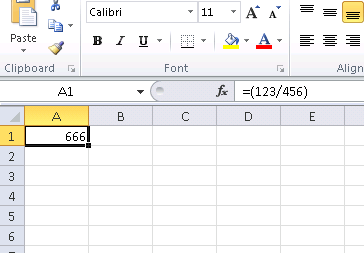
\includegraphics[scale=0.66]{digging_into_code/Excel_prank.png}
\caption{\IFRU{Пранк сработал}{Practical joke worked}}
\end{figure}

\IFRU{Если попробовать ту же версию Excel, только x64, то окажется что там инструкций \FDIV всего 12, 
причем нужная нам ~--- третья по счету.}
{If to try the same Excel version, but x64, we'll see there are only 12 \FDIV instructions,
and the one we looking for ~--- third.}

\begin{lstlisting}
gt64.exe -l:excel.exe bpx=excel.exe!base+0x1B7FCC,set(st0,666)
\end{lstlisting}

\IFRU{Видимо, все дело в том что много операций деления переменных типов \Tfloat и \Tdouble 
компилятор заменил на SSE-инструкции вроде \TT{DIVSD}, 
коих здесь теперь действительно много (\TT{DIVSD} присутствует в количестве 268 инструкций).}
{It seems, a lot of division operations of \Tfloat and \Tdouble types, compiler replaced by SSE-instructions
like \TT{DIVSD} (\TT{DIVSD} present here 268 in total).}

\section{\IFRU{Подозрительные паттерны кода}{Suspicious code patterns}}

\IFRU{Современные компиляторы не генерируют инструкции \TT{LOOP} и \TT{RCL}. 
С другой стороны, эти инструкции хорошо знакомы кодерам предпочитающим писать прямо на ассемблере. 
Если такие инструкции встретились, можно сказать с какой-то вероятностью, что этот кусок кода написан вручную.}
{Modern compilers do not emit \TT{LOOP} and \TT{RCL} instructions.
On the other hand, these instructions are well-known to coders who like to code in straight assembler.
If you spot these, it can be said, with a big probability, this piece of code is hand-written.}
% TODO: also, function prologue/epilogue isn't present
